\documentclass{article}
\usepackage[utf8]{inputenc}

\usepackage{amsmath}
\usepackage{amssymb}
\usepackage[top=1in, bottom=1in, left=1in, right=1in]{geometry}

\usepackage{multicol}

\usepackage{tikz}
\usepackage{pgfplots}

\usepackage{float}
\usepackage{caption}

\setlength{\parindent}{0em}
\setlength{\parskip}{1em}

\title{EECS 560 - Lab \#6}
\author{Theodore Lindsey}

\date{October 16, 2015}

\begin{document}

\maketitle


\section{Overall Organization of Experiment}

For this lab, we attempt to evaluate whether hashing with open addressing or hashing with chaining performs more quickly provided the same records are inserted into both tables.




\section{Data Generation}

In this experiment, it is necessary that we insert the same values into both the hash table with open addressing and the hash table with chaining in order to achieve an apple-to-apples comparison.  To this end, we will use identical seeds for our pseudo random number generator in order to ensure that the same sequence of ``random'' numbers are inserted into both tables.

In order to reduce variation in the results, multiple trials are run for each load factor.  Each trial uses a different seed in order to reduce the impact of troublesome values to be inserted that might occur from a particular seed.  Each of the seeds used is the same for corresponding trials in each load factor group.

Timing is measured by the provided timer class.  Times for individual runs are not printed to the console but are recorded in the log file (`log.csv').  Averages for a specific load factor and hashing type are printed to the console but not recorded in the log file since they can easily be re-calculated from the log file as needed.




\section{Summary of Results (CPU Timing)}

In all trials, the hash table with open addressing had better performance than the corresponding hash table with chaining.  Running 100 seed trials per load factor produced essentially the same average results as running 5 seed trials per load factor (as seen in Figure \ref{fig:5_seeds} and Figure \ref{fig:100_seeds}) which suggests that the observed timings are consistent and representative of both table's general performance for the tested load factors.




\section{Observation and Conclusion}

From the data, it appears clear that the hash table with open addressing consistently performs better than the hash table with chaining.  This is likely due to the fact that there is less overhead to look at the next element in an array than there is to look through a linked list.

Additionally, as expected, the time to finish the insertions increases as the load increases.  Also, the rate at which the completion time increases is more than linear.  This is consistent with the fact that as more data is inserted into the table, the likelihood of a collision increases and since dealing with a collision takes more time than simply computing a hash, performance is negativly affected.




\section{Data}

Figure \ref{tab:5_seeds} shows the results of the experiment.  Timing results for open addressing and chaining are directly compared for each load factor and seed.  Then, for each load factor, all of the times for open addressing are averaged and all of the times for chaining are averaged.
\begin{figure}[H]
\centering
\begin{tabular}{|cccc|cccc|cccc|}\hline
LF & Seed & Open & Chain & LF & Seed & Open & Chain & LF & Seed & Open & Chain  \\ \hline
0.2 & 0 & 0.02638 & 0.04925 & 0.3 & 0 & 0.02929 & 0.04941 & 0.4 & 0 & 0.03406 & 0.05386 \\
0.2 & 1 & 0.01743 & 0.02698 & 0.3 & 1 & 0.02567 & 0.04037 & 0.4 & 1 & 0.03452 & 0.05337 \\
0.2 & 2 & 0.01744 & 0.02699 & 0.3 & 2 & 0.02571 & 0.04015 & 0.4 & 2 & 0.03408 & 0.05392 \\
0.2 & 3 & 0.01743 & 0.02702 & 0.3 & 3 & 0.02565 & 0.04017 & 0.4 & 3 & 0.03454 & 0.05390 \\
0.2 & 4 & 0.01743 & 0.02699 & 0.3 & 4 & 0.02583 & 0.03973 & 0.4 & 4 & 0.03454 & 0.05389 \\
\multicolumn{2}{|c}{\textbf{avg}} & \textbf{0.01922} & \textbf{0.03145} & \multicolumn{2}{|c}{\textbf{avg}} & \textbf{0.02643} & \textbf{0.04196} & \multicolumn{2}{|c}{\textbf{avg}} & \textbf{0.03435} & \textbf{0.05379} \\ \hline
0.5 & 0 & 0.04432 & 0.06880 & 0.6 & 0 & 0.05536 & 0.08335 & 0.7 & 0 & 0.07458 & 0.10260 \\
0.5 & 1 & 0.04436 & 0.06848 & 0.6 & 1 & 0.05539 & 0.08346 & 0.7 & 1 & 0.06858 & 0.09924 \\
0.5 & 2 & 0.04434 & 0.06815 & 0.6 & 2 & 0.05539 & 0.08329 & 0.7 & 2 & 0.06766 & 0.09832 \\
0.5 & 3 & 0.04426 & 0.06813 & 0.6 & 3 & 0.05533 & 0.08793 & 0.7 & 3 & 0.06766 & 0.09918 \\
0.5 & 4 & 0.04449 & 0.06818 & 0.6 & 4 & 0.05550 & 0.08319 & 0.7 & 4 & 0.06858 & 0.09925 \\
\multicolumn{2}{|c}{\textbf{avg}} & \textbf{0.04435} & \textbf{0.06835} & \multicolumn{2}{|c}{\textbf{avg}} & \textbf{0.05539} & \textbf{0.08424} & \multicolumn{2}{|c}{\textbf{avg}} & \textbf{0.06941} & \textbf{0.09972} \\ \hline
\end{tabular}
\caption{Times with 5 seed trials per load factor}
\label{tab:5_seeds}
\end{figure}

Figure \ref{tab:100_seeds} shows the average time to completion for each method for each load factor.  There are too many data points to show the results for each individual trial.

\begin{figure}[H]
\centering
\begin{tabular}{|l|llllll|}\hline
Load factor               & 0.2       & 0.3       & 0.4       & 0.5       & 0.6       & 0.7       \\ \hline
Average (open addressing) & 0.0201543 & 0.0256411 & 0.0343655 & 0.0442488 & 0.0558289 & 0.0686431 \\
Average (chaining)        & 0.0304140 & 0.0402859 & 0.0539557 & 0.0684946 & 0.0845346 & 0.0995307 \\ \hline
\end{tabular}
\caption{Times with 100 seed trials per load factor}
\label{tab:100_seeds}
\end{figure}




\section{Visualisation of Data}

Figure \ref{fig:5_seeds} shows the average completion times for each load factor when 5 seed trials were performed.  I was curious how reliable the results were so I followed up the 5 seed trials per load factor with an additional experiment in which I used 100 seed trials per load factor, as seen in Figure \ref{fig:100_seeds}.  As is see by comparing the figures, the results gathered from only 5 seed trials per load factor appear to be quite reliable and representative of the general performance of each hashing method.

\begin{figure}[H]
\centering

\begin{minipage}{0.45\textwidth}
    \centering
    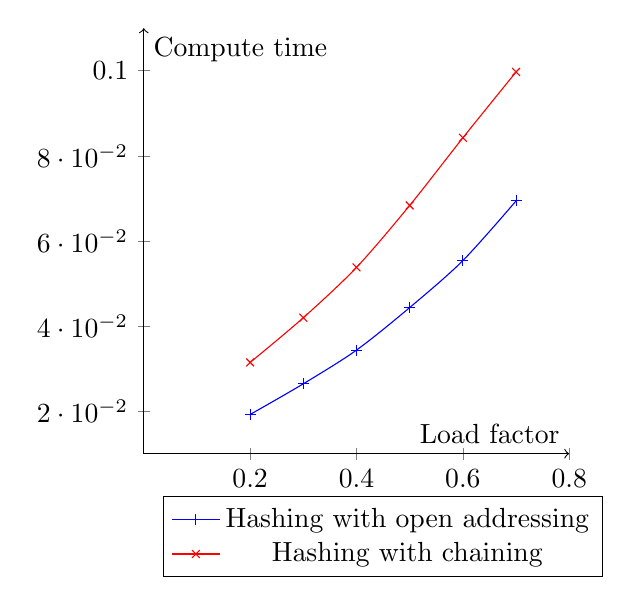
\begin{tikzpicture}
        \begin{axis}[
            width=2.75in,
            height=2.75in,
            xmin=0,
            xmax=0.8,
            ymin=0.01,
            ymax=0.11,
            axis lines=middle,
            axis line style={->},
            xlabel=Load factor,
            ylabel=Compute time,
            legend style={at={(axis cs:0.45,0.0)},anchor=north}]
            
        \addplot[smooth,blue,mark=+] plot coordinates {
            (0.2,0.01922)
            (0.3,0.02643)
            (0.4,0.03435)
            (0.5,0.04435)
            (0.6,0.05539)
            (0.7,0.06941)
        };
        \addlegendentry{Hashing with open addressing}
    
        \addplot[smooth,color=red,mark=x] plot coordinates {
            (0.2,0.03145)
            (0.3,0.04196)
            (0.4,0.05379)
            (0.5,0.06835)
            (0.6,0.08424)
            (0.7,0.09972)
        };
        \addlegendentry{Hashing with chaining}
        \end{axis}
    \end{tikzpicture}
    \captionof{figure}{5 seeds per load factor.}
    \label{fig:5_seeds}
\end{minipage}
\begin{minipage}{0.45\textwidth}
    \centering
    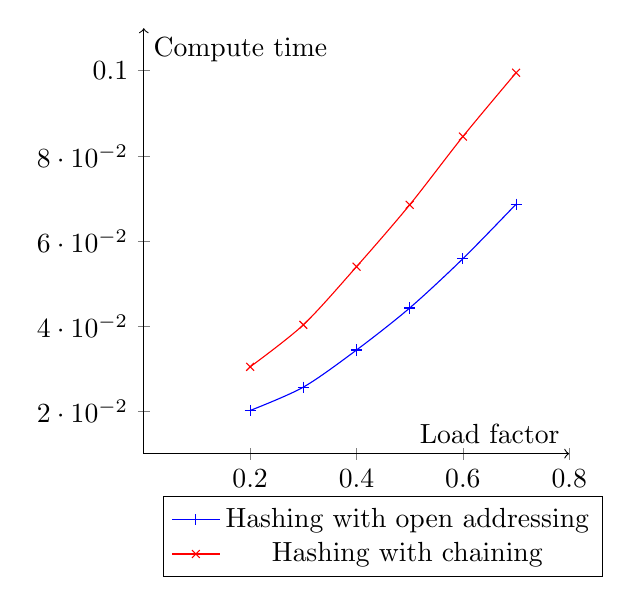
\begin{tikzpicture}
        \begin{axis}[
            width=2.75in,
            height=2.75in,
            xmin=0,
            xmax=0.8,
            ymin=0.01,
            ymax=0.11,
            axis lines=middle,
            axis line style={->},
            xlabel=Load factor,
            ylabel=Compute time,
            legend style={at={(axis cs:0.45,0.0)},anchor=north}]
            
        \addplot[smooth,blue,mark=+] plot coordinates {
            (0.2,0.0201543)
            (0.3,0.0256411)
            (0.4,0.0343655)
            (0.5,0.0442488)
            (0.6,0.0558289)
            (0.7,0.0686431)
        };
        \addlegendentry{Hashing with open addressing}
    
        \addplot[smooth,color=red,mark=x] plot coordinates {
            (0.2,0.0304140)
            (0.3,0.0402859)
            (0.4,0.0539557)
            (0.5,0.0684946)
            (0.6,0.0845346)
            (0.7,0.0995307)
        };
        \addlegendentry{Hashing with chaining}
        \end{axis}
    \end{tikzpicture}
    \captionof{figure}{100 seeds per load factor.}
    \label{fig:100_seeds}
\end{minipage}
\end{figure}
    



\end{document}